\documentclass[a4paper, 12pt]{book}

\usepackage[utf8x]{inputenc}   % omogoča uporabo slovenskih črk kodiranih v formatu UTF-8
\usepackage[slovene,english]{babel}    % naloži, med drugim, slovenske delilne vzorce
\usepackage[pdftex]{graphicx}  % omogoča vlaganje slik različnih formatov
\usepackage{fancyhdr}          % poskrbi, na primer, za glave strani
\usepackage{amssymb}           % dodatni simboli
\usepackage{amsmath}           % eqref, npr.
%\usepackage{hyperxmp}
\usepackage[hyphens]{url}  % dodal Solina
\usepackage{comment}       % dodal Solina

\usepackage[pdftex, colorlinks=true,
						citecolor=black, filecolor=black, 
						linkcolor=black, urlcolor=black,
						pagebackref=false, 
						pdfproducer={LaTeX}, pdfcreator={LaTeX}, hidelinks]{hyperref}

\usepackage{color}      
\usepackage{soul} 
\usepackage[numbers]{natbib}

%%%%%%%%%%%%%%%%%%%%%%%%%%%%%%%%%%%%%%%%
%	DIPLOMA INFO
%%%%%%%%%%%%%%%%%%%%%%%%%%%%%%%%%%%%%%%%
% \newcommand{\fixspacing}{\vspace{0pt plus 1filll}\mbox{}}

\newcommand{\ttitle}{Različni pristopi umetne inteligence v video igrah}
\newcommand{\ttitleEn}{Different Artificial intelligence approaches in video games}
\newcommand{\tsubject}{\ttitle}
\newcommand{\tsubjectEn}{\ttitleEn}
\newcommand{\tauthor}{Jovan Prodanov}
\newcommand{\tkeywords}{računalniška igra, umetna inteligenca, računalnik, pristopi}
\newcommand{\tkeywordsEn}{computer game, artificial intelligence, computer, approaches}

\usepackage{hyperref}
%%%%%%%%%%%%%%%%%%%%%%%%%%%%%%%%%%%%%%%%
%	HYPERREF SETUP
%%%%%%%%%%%%%%%%%%%%%%%%%%%%%%%%%%%%%%%%
\hypersetup{pdftitle={\ttitle}}
\hypersetup{pdfsubject=\ttitleEn}
\hypersetup{pdfauthor={\tauthor, jp6957@student.uni-lj.si}}
\hypersetup{pdfkeywords=\tkeywordsEn}

%%%%%%%%%%%%%%%%%%%%%%%%%%%%%%%%%%%%%%%%
% PAGE SETUP
%%%%%%%%%%%%%%%%%%%%%%%%%%%%%%%%%%%%%%%% 
\addtolength{\marginparwidth}{-20pt} % robovi za tisk
\addtolength{\oddsidemargin}{40pt}
\addtolength{\evensidemargin}{-40pt}

\renewcommand{\baselinestretch}{1.3} % ustrezen razmik med vrsticami
\setlength{\headheight}{15pt}        % potreben prostor na vrhu
\renewcommand{\chaptermark}[1]
{\markboth{\MakeUppercase{\thechapter.\ #1}}{}} \renewcommand{\sectionmark}[1]
{\markright{\MakeUppercase{\thesection.\ #1}}} \renewcommand{\headrulewidth}{0.5pt} \renewcommand{\footrulewidth}{0pt}
\fancyhf{}
\fancyhead[LE,RO]{\sl \thepage} 
%\fancyhead[LO]{\sl \rightmark} \fancyhead[RE]{\sl \leftmark}
\fancyhead[RE]{\sc \tauthor}              % dodal Solina
\fancyhead[LO]{\sc Bachelor's thesis}     % dodal Solina

\newcommand{\BibTeX}{{\sc Bib}\TeX}

%%%%%%%%%%%%%%%%%%%%%%%%%%%%%%%%%%%%%%%%
% TITLES
%%%%%%%%%%%%%%%%%%%%%%%%%%%%%%%%%%%%%%%%  
\newcommand{\autfont}{\Large}
\newcommand{\titfont}{\LARGE\bf}
\newcommand{\clearemptydoublepage}{\newpage{\pagestyle{empty}\cleardoublepage}}
\setcounter{tocdepth}{1}	      % globina kazala

%%%%%%%%%%%%%%%%%%%%%%%%%%%%%%%%%%%%%%%%
% CONSTRUCTORS
%%%%%%%%%%%%%%%%%%%%%%%%%%%%%%%%%%%%%%%%  
% \newtheorem{izrek}{Izrek}[chapter]
% \newtheorem{trditev}{Trditev}[izrek]
% \newenvironment{dokaz}{\emph{Dokaz.}\ }{\hspace{\fill}{$\Box$}}

%%%%%%%%%%%%%%%%%%%%%%%%%%%%%%%%%%%%%%%%%%%%%%%%%%%%%%%%%%%%%%%%%%%%%%%%%%%%%%%
%% PDF-A
%%%%%%%%%%%%%%%%%%%%%%%%%%%%%%%%%%%%%%%%%%%%%%%%%%%%%%%%%%%%%%%%%%%%%%%%%%%%%%%

%%%%%%%%%%%%%%%%%%%%%%%%%%%%%%%%%%%%%%%% 
% define medatata
%%%%%%%%%%%%%%%%%%%%%%%%%%%%%%%%%%%%%%%% 
\def\Title{\ttitle}
\def\Author{\tauthor, ales.jaklic@fri.uni-lj.si}
\def\Subject{\ttitleEn}
\def\Keywords{\tkeywordsEn}

%%%%%%%%%%%%%%%%%%%%%%%%%%%%%%%%%%%%%%%% 
% \convertDate converts D:20080419103507+02'00' to 2008-04-19T10:35:07+02:00
%%%%%%%%%%%%%%%%%%%%%%%%%%%%%%%%%%%%%%%% 
\def\convertDate{%
    \getYear
}

{\catcode`\D=12
 \gdef\getYear D:#1#2#3#4{\edef\xYear{#1#2#3#4}\getMonth}
}
\def\getMonth#1#2{\edef\xMonth{#1#2}\getDay}
\def\getDay#1#2{\edef\xDay{#1#2}\getHour}
\def\getHour#1#2{\edef\xHour{#1#2}\getMin}
\def\getMin#1#2{\edef\xMin{#1#2}\getSec}
\def\getSec#1#2{\edef\xSec{#1#2}\getTZh}
\def\getTZh +#1#2{\edef\xTZh{#1#2}\getTZm}
\def\getTZm '#1#2'{%
    \edef\xTZm{#1#2}%
    \edef\convDate{\xYear-\xMonth-\xDay T\xHour:\xMin:\xSec+\xTZh:\xTZm}%
}

%\expandafter\convertDate\pdfcreationdate 

%%%%%%%%%%%%%%%%%%%%%%%%%%%%%%%%%%%%%%%%
% get pdftex version string
%%%%%%%%%%%%%%%%%%%%%%%%%%%%%%%%%%%%%%%% 
\newcount\countA
\countA=\pdftexversion
\advance \countA by -100
\def\pdftexVersionStr{pdfTeX-1.\the\countA.\pdftexrevision}


%%%%%%%%%%%%%%%%%%%%%%%%%%%%%%%%%%%%%%%%
% XMP data
%%%%%%%%%%%%%%%%%%%%%%%%%%%%%%%%%%%%%%%%  
\usepackage{xmpincl}
%\includexmp{pdfa-1b}

%%%%%%%%%%%%%%%%%%%%%%%%%%%%%%%%%%%%%%%%
% pdfInfo
%%%%%%%%%%%%%%%%%%%%%%%%%%%%%%%%%%%%%%%%  
\pdfinfo{%
    /Title    (\ttitle)
    /Author   (\tauthor, jp6957@student.uni-lj.si)
    /Subject  (\ttitleEn)
    /Keywords (\tkeywordsEn)
    /ModDate  (\pdfcreationdate)
    /Trapped  /False
}


%%%%%%%%%%%%%%%%%%%%%%%%%%%%%%%%%%%%%%%
% START
%%%%%%%%%%%%%%%%%%%%%%%%%%%%%%%%%%%%%%%
\begin{document}
\selectlanguage{english}
\frontmatter
\setcounter{page}{1} %
\renewcommand{\thepage}{}       % preprecimo težave s številkami strani v kazalu
\newcommand{\sn}[1]{"`#1"'}                    % dodal Solina (slovenski narekovaji)

%%%%%%%%%%%%%%%%%%%%%%%%%%%%%%%%%%%%%%%%
% INTRO
%%%%%%%%%%%%%%%%%%%%%%%%%%%%%%%%%%%%%%%%
 \thispagestyle{empty}%
   \begin{center}
    {\large\sc Univerza v Ljubljani\\%
      Fakulteta za računalništvo in informatiko}%
    \vskip 10em%
    {\autfont \tauthor\par}%
    {\titfont \ttitle \par}%
    {\vskip 2em \textsc{DIPLOMSKO DELO\\[2mm]
    VISOKOŠOLSKI STROKOVNI ŠTUDIJSKI PROGRAM PRVE STOPNJE RAČUNALNIŠTVO IN INFORMATIKA}\par}%
    \vfill\null%
    {\large \textsc{Mentor}: doc.\ dr.  Aleš Jaklič\par}%
    {\vskip 2em \large Ljubljana, 2022 \par}%
\end{center}

\clearemptydoublepage

%%%%%%%%%%%%%%%%%%%%%%%%%%%%%%%%%%%%%%%%
% INTRO ENGLISH
%%%%%%%%%%%%%%%%%%%%%%%%%%%%%%%%%%%%%%%%
 \thispagestyle{empty}%
   \begin{center}
    {\large\sc University of Ljubljana\\%
      Faculty of Computer and Information Science}%
    \vskip 10em%
    {\autfont \tauthor\par}%
    {\titfont \ttitleEn \par}%
    {\vskip 2em \textsc{Bachelor's Thesis\\[2mm]
    UNIVERSITY STUDY PROGRAMME UNDERGRADUATE PROGRAMMES COMPUTER AND INFORMATION SCIENCE}\par}%
    % Not sure if correct "University"
    \vfill\null%
    {\large \textsc{Mentor}: doc.\ dr.  Aleš Jaklič\par}%
    {\vskip 2em \large Ljubljana, 2022 \par}%
\end{center}


%%%%%%%%%%%%%%%%%%%%%%%%%%%%%%%%%%%%%%%%
% copyright page
%%%%%%%%%%%%%%%%%%%%%%%%%%%%%%%%%%%%%%%%
\thispagestyle{empty}
\vspace*{8cm}

\noindent
{\sc Copyright}. 
Rezultati diplomske naloge so intelektualna lastnina avtorja in matične fakultete Univerze v Ljubljani.
Za objavo in koriščenje rezultatov diplomske naloge je potrebno pisno privoljenje avtorja, fakultete ter mentorja.

\begin{center}
\mbox{}\vfill
\emph{Besedilo je oblikovano z urejevalnikom besedil \LaTeX.}
\end{center}
%%%%%%%%%%%%%%%%%%%%%%%%%%%%%%%%%%%%%%%%

\clearemptydoublepage

%%%%%%%%%%%%%%%%%%%%%%%%%%%%%%%%%%%%%%%%
% stran 3 med uvodnimi listi
\thispagestyle{empty}
\
\vfill

\bigskip
\noindent\textbf{Kandidat:} \tauthor\\
\noindent\textbf{Naslov:} \ttitle\\
\noindent\textbf{Vrsta naloge:} Diplomska naloga na visokošolskem programu prve stopnje Računalništvo in informatika \\
\noindent\textbf{Mentor:} doc. dr. Aleš Jaklič\\

\bigskip
\noindent\textbf{Opis:}\\
Raziskovanje različnih načinov uporabe umetne inteligence v računalniški igri. Od osnovnih stanj do algoritmov strojnega učenja. Cilj je poskušati primerjati rezultate različnih metod in ugotoviti najboljše.\\
Besedilo teme diplomskega dela študent prepiše iz študijskega informacijskega sistema, kamor ga je vnesel mentor. 
V nekaj stavkih bo opisal, kaj pričakuje od kandidatovega diplomskega dela. 
Kaj so cilji, kakšne metode naj uporabi, morda bo zapisal tudi ključno literaturo.

\bigskip
\noindent\textbf{Title:} \ttitleEn

\bigskip
\noindent\textbf{Description:}\\
Researching different ways of how Artificial intelligence is used in a computer game. From basic state machines to machine learning algorithms. The goal is trying to compare results of different methods and figure out the best ones.


\vfill

\vspace{2cm}

% prazna stran
\clearemptydoublepage

% zahvala
\thispagestyle{empty}\mbox{}\vfill\null\it%
\noindent
Zelo sem hvaležen vsem, ki so mi pomagali priti tja, kjer sem.
\rm\normalfont

% prazna stran
\clearemptydoublepage

%%%%%%%%%%%%%%%%%%%%%%%%%%%%%%%%%%%%%%%%
% posvetilo, če sama zahvala ne zadošča :-)
%%%%%%%%%%%%%%%%%%%%%%%%%%%%%%%%%%%%%%%%

\thispagestyle{empty}\mbox{}{\vskip0.20\textheight}\mbox{}\hfill\begin{minipage}{0.55\textwidth}%
Za svoja draga družina.
\normalfont\end{minipage}

% prazna stran
\clearemptydoublepage


%%%%%%%%%%%%%%%%%%%%%%%%%%%%%%%%%%%%%%%%
% kazalo
\pagestyle{empty}
\def\thepage{}% preprecimo tezave s stevilkami strani v kazalu
\tableofcontents{}


% prazna stran
\clearemptydoublepage


%%%%%%%%%%%%%%%%%%%%%%%%%%%%%%%%%%%%%%%%
% List of abbriviations
%%%%%%%%%%%%%%%%%%%%%%%%%%%%%%%%%%%%%%%%

% \chapter*{Seznam uporabljenih kratic}  % spremenil Solina, da predolge vrstice ne gredo preko desnega roba
\chapter*{List of abbreviations used}  % spremenil Solina, da predolge vrstice ne gredo preko desnega roba

\noindent\begin{tabular}{p{0.21\textwidth}|p{.4\textwidth}|p{.4\textwidth}}    % po potrebi razširi prvo kolono tabele na račun drugih dveh!
    % {\bf kratica} & {\bf angleško} & {\bf slovensko} \\ \hline
  {\bf Abbreviation} & {\bf English} & {\bf Slovenian} \\ \hline
  % after \\: \hline or \cline{col1-col2} \cline{col3-col4} ...
  {\bf ML}      & machine learning                  & strojno učenje \\
  {\bf FSM}     & finite state machine              & končni stroj \\
  {\bf NN}      & neural network                    & nevronska mreža \\
  {\bf CNN}     & convolutional neural network      & konvolucijska nevronska mreža \\
  {\bf NPC}     & non-player character              & neigralski lik \\
  {\bf CA}      & classification accuracy           & klasifikacijska točnost \\
  {\bf BF }     & behaviour trees                   & drevesa vedenja \\
  \dots         & \dots                             & \dots \\
\end{tabular}

% prazna stran
\clearemptydoublepage

%%%%%%%%%%%%%%%%%%%%%%%%%%%%%%%%%%%%%%%%
% povzetek
%%%%%%%%%%%%%%%%%%%%%%%%%%%%%%%%%%%%%%%%

\addcontentsline{toc}{chapter}{Povzetek}
\chapter*{Povzetek}

\noindent\textbf{Naslov:} \ttitle
\bigskip

\noindent\textbf{Avtor:} \tauthor
\bigskip

%\noindent\textbf{Povzetek:} 
\noindent 
V diplomski nalogi bodo predstavljeni različni načini uporabe umetne inteligence v računalniških igrah s poudarkom na orodju, ki deep reinforcement learning.
Ta diplomska naloga bo obravnavala načine ravnanja z umetno inteligenco v video igrah, kot so: FMS, mehka logika, skriptiranje, zbiranje, drevesa odločanja, vedenjska drevesa, nevronske mreže, genetski algoritmi.
Raziskoval bom zgoraj omenjene načine, naredil primere in predstavil njihove rezultate.
\bigskip

\noindent\textbf{Ključne besede:} \tkeywords.
% prazna stran
\clearemptydoublepage


%%%%%%%%%%%%%%%%%%%%%%%%%%%%%%%%%%%%%%%%
% abstract
%%%%%%%%%%%%%%%%%%%%%%%%%%%%%%%%%%%%%%%%

\selectlanguage{english}
\addcontentsline{toc}{chapter}{Abstract}
\chapter*{Abstract}

\noindent\textbf{Title:} \ttitleEn
\bigskip

\noindent\textbf{Author:} \tauthor
\bigskip

%\noindent\textbf{Abstract:} 
\noindent 
The thesis will present different ways of using artificial intelligence in computer games with an emphasis on a tool that uses deep reinforcement learning.
This thesis will handle ways of handling AI in video games like: FMS, Fuzzy logic, Scripting, Flocking, Decision trees, Behavioural trees, Neural networks, Genetics Algorithm.
I will research the above aforementioned ways, even make examples and present their results.
\bigskip



\noindent\textbf{Keywords:} \tkeywordsEn.
\selectlanguage{english}
% prazna stran
\clearemptydoublepage


%%%%%%%%%%%%%%%%%%%%%%%%%%%%%%%%%%%%%%%%
% START
%%%%%%%%%%%%%%%%%%%%%%%%%%%%%%%%%%%%%%%%

\mainmatter
\setcounter{page}{1}
\pagestyle{fancy}


\chapter{Introduction}

As soon as the first video game arrived, there was a wish, no, a need to create a more involving experience. So, game developers created game AI to let the player interact with the game on so many levels.

Creating an AI in video games comes with its own problems, in this thesis we will take our time to explain some techniques and their downfalls. We will also take a look into the future of the progression of game AI.


In chapter \ref{ch1} we are going to get introduced with the problem and its intricacies. Chapter \ref{ch2} will take a tour through a number of techniques developers created through the times for solving game AI. But, in chapter \ref{ch3} I will present a "newer" experimental techniques and give out my conclusion in chapter \ref{ch4}.


\chapter{Background}
\label{ch1}
The question of game AI was present even in the first of games developed. By definition, in video games, AI is used to generate responsive, adaptive or intelligent behaviors primarily in NPCs similar to human-like intelligence \cite{AIwiki}. The ways of approaching it is incredibly vast, in this thesis we will only scratch the surface, but focus on the most interesting ones.

\section{What is AI in games?}
First, I should start with the term "video game", in definition it is an electronic game that involves interaction with a user interface or input device such as a joystick, controller, keyboard, or motion sensing device to generate visual feedback \cite{VideoGameWiki}. Then, the visual feedback is channeled to a displaying device, which can be observed. 

So, now for quite some time, game developers are trying to invent techniques and methods for incorporating intelligence into these video games. But, this AI is a broad term, in video games, it can mean: animation control, steering, flocking, pathfinding, planning, procedural generation, tactical and strategic thinking, learning \cite{FuzzyAIGames}, to name a few. Often game AI can be mistaken for "true AI", which is to display human cognitive skills associated with human thinking, learning and problem-solving.

Game AI adds another piece of the puzzle of defining AI and that is the illusion of intelligence. We would never want in a game an unbeatable ever-learning opponent, we would like a fun and easy experience, which isn't obviously stupid. Game AI in video games exists only to be fun and entertaining, so looking from this point, this is why the game developers are sticking to things that are predictable and working and aren't experimenting a whole lot, because who would want unexpected things happening in a game.

\section{Illusion of intelligence}
Now that the secret is out, game developers were and are inventing tricks and techniques to make the player believe that games have real intelligence \cite{IllusionOfIntelligece}. And instead of making the goal true intelligence, its the appearance of intelligence.

\subsection{Why does it work?}
The true reason why this illusion works is that players want to believe that there are glimmers of real human-like intelligence in their virtual worlds \cite{IllusionOfIntelligece}. Also, with their high expectations the players are easily forgiving.

Another reason why it works is because of anthropomorphism, which is an attribution of human motivation, characteristics, or behavior to inanimate objects, animals, or natural phenomenon, and these can be related to a phenomenon in animation. There is a research that a preschool 91\% of the times picked a character that is not a human being 
 \cite{AnthropomorphicCharacters}.

As previously stated, expectations have a high influence. Because of the placebo effect, if players are expecting a highly intelligent game, their enjoyment will be higher. This is the same as if people think they are eating a more expensive food or a drink, they are more likely to enjoy it.

\subsection{Selling it}
The illusion of intelligence work when there is a certain level of quality to it, and that quality is helped by \cite{IllusionOfIntelligece}:
\begin{itemize}
    \item The AI should have \emph{animation and dialog}. These things help it to interact with the world and player, as well as making it more alive and present.
    \item Although animations help to achieve game AI, it should be done with quality. They should the smooth and human-like, instead of looking like a \emph{robot}.
    \item \emph{Have a reason to exist}, AI characters shouldn't always wait for the player to approach, they should have their own purpose. As well as their own motives, because the game world would be their home and reality and they should have their own states in it.
    \item The culmination of building a successful AI character would be for it to have its own \emph{personality}. How the game developer leverages this powerful tool can complete change the feel of the game.
\end{itemize}


\section{Deterministic vs Non-deterministic}
It is in close connection to game AI that there exists two type of games. In a deterministic game, the course of the game depends only on the players’ decisions, but in a non-deterministic game, there’s some factor of randomness involved \cite{DeepLearningGO}.

For example, chess is a deterministic game, the outcome of the game is entirely based on the players' decisions. But, football is non-deterministic, the players can't reliably kick the ball exactly the same every time. In that sense, luck or randomness often makes the game more exciting, however too much randomness removes all influence of the player in game, which is rarely fun.


\chapter{Current AI in games}
\label{ch2}

So, advanced techniques for game AI have been spotted more often, for examples, there have been usages of Bayesian networks and neural networks for real-time strategy games, as well as evolutionary algorithms \cite{FuzzyAIGames}. But, in those cases the game seems to orbit around that as the main focus of the game itself. In other words, advanced techniques for game AI currently need a game to be build around them. Then, there is the problem of evolutionary algorithms needing a high computational and memory power. Also, the last problem would be their non-determinism, that just brings more problems to the table and game developers are reluctant to ship a game that is not tested enough.

In this chapter, we will focus more on the current techniques that are widely used, which finely sell the illusion of intelligence. Technologies I will use if I need to present examples are Unity for the game editor and game engine \cite{UnitySoftware}.

\section{Finite State Machines}

You want to create a side-scrolling platformer, and now you grab a pen and paper and start designing the flowchart. You draw a box for everything the hero can be doing: standing, jumping, ducking and diving. When some kind of input is given, for an example when a button is pressed, you draw an arrow to from that box, label it with the button, and connect it to the box it changes to \cite{GameProgrammingPattersFMS}.

\begin{figure}[h]
\begin{center}
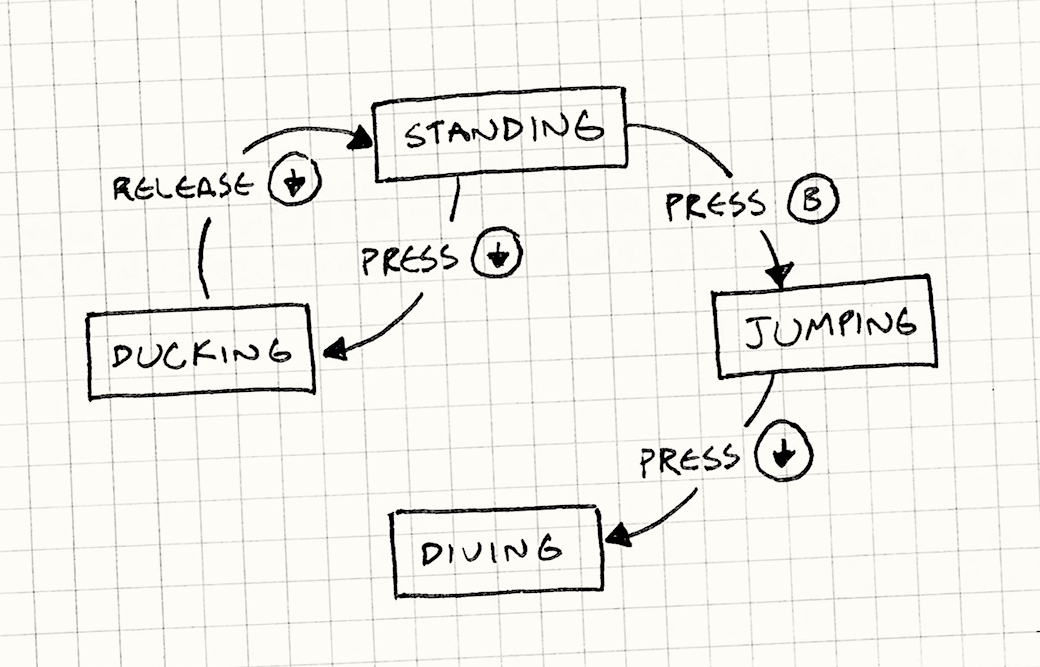
\includegraphics[width=0.5\textwidth]{Images/state_FSM.png}
\end{center}
\caption{Finite State Machine}
\label{pic1}
\end{figure}

Now that we successfully create a FSM, these came out of a computer science branch called automata theory, which includes the famous Turing machine. FSMs are the simplest of that bunch.

\begin{itemize}
    \item You have to have fixed set of states the machine can be in
    \item The machine can be in one state at a time
    \item Sequences of inputs or events are being sent to the machine
    \item Each state has a set of transitions, each associated  with an input/event and pointing to a state
\end{itemize}

So, now that I've introduced FSMs, there is a catch. State machines help you untangle hairy code by forcing a very constrained structure on it. All you have is a fixed set of states, a single current state, and some hardcoded transitions \cite{GameProgrammingPattersFMS}. However, when wanting to create a more complex game AI, you have to work around these problems, I'll close this chapter by presenting some. 

\subsection{Concurrent State Machines}

Let's now equip our hero with a gun. If we want to play by the constraints of an FSM, we have to double our states: standing, standing with a gun, jumping, jumping with a gun etc. Its redundant, however we can add another state into a single machine, what the hero is doing and what he's carrying.

\begin{verbatim}
class Hero  {
    private State _state;
    private State _equipment;

    private void HandleInput(Input input) {
        _state.HandleInput(input);
        _equipment.HandleInput(input);
    }
}
\end{verbatim}

\subsection{Hierarchical State Machines}

We wouldn't want to duplicate code in all of our states. We could define a state "on ground" that handles ducking and jumping, standing, walking, running would then inherit from that one and add it to its own behaviour.

Turns out this is a structure called hierarchical state machine, a state can have a superstate (making itself a substate). When an event comes in, if the substate doesn’t handle it, it rolls up the chain of superstates. In other words, it works just like overriding inherited methods \cite{GameProgrammingPattersFMS}.

If the current state is on top of the stack, under that is its superstate and so on. So, if you dish out a state-specific behaviour, it starts on top of the stack and walks down until one of the superstates handles it, but if none do, its ignored.

\subsection{Pushdown Automata}

This is an extension to FSM, that uses the concept of stacks. The problem is with basic FSMs is that you don't have history of the previous states. You know of what state you \emph{are} currenly in, but no memory of what state you \emph{were}.

So, if we had states standing and firing, if we were to transition in the firing state, we couldn't remember to go in our previous state, the standing state. For this problem, the pushdown automata structure is here to help.

In vanilla FSM, you have a singe pointer to the current state, pushdown automata has a stack of them. In a FSM, transitioning into the new state replaces the previous one. Pushdown automata let's you do that, but it gives you two other choices \cite{GameProgrammingPattersFMS}:

\begin{itemize}
    \item You can push a new state on the stack, the "current" state is always on top of the stack, so this transitions to the new state, but it leaves the previous state directly under the stack instead of discrading.
    \item You can pop the "current" state, in doing so, the state that is under it becomes the new "current" state.
\end{itemize}

\begin{figure}[h]
\begin{center}
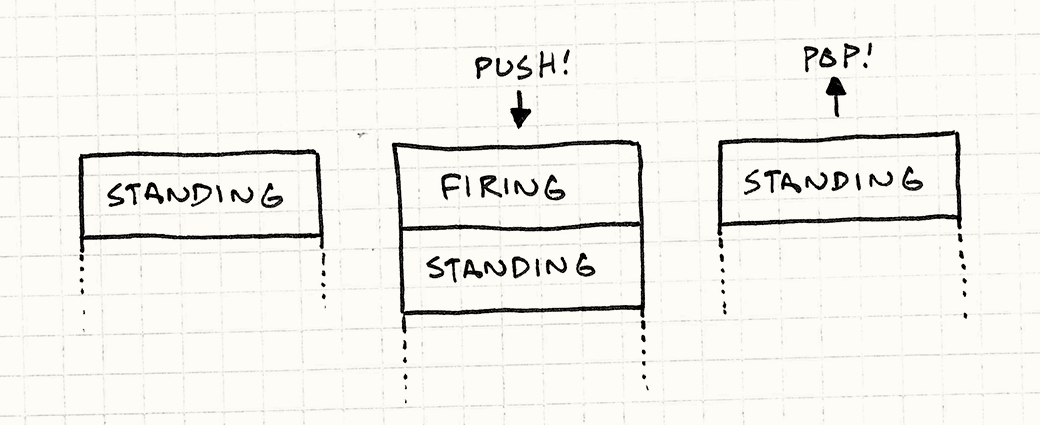
\includegraphics[width=0.6\textwidth]{Images/state_pushdown.png}
\end{center}
\caption{The Pushdown Automata}
\label{pic2}
\end{figure}

\section{Behaviour Trees}

Even with extensions to FSMs, they are pretty limited. If the aim is complex game AI, the previous chapter only whet our appetite.

Behaviour trees (BTs) are a proven and established technique that game developers regularly use to build their AI. Not only do they give you a solid foundation to build upon, but it also gives you a lot of flexibility to include other techniques in a way that gives you full control over behavior and performance \cite{BehaviourTreeStarterPack}.

So, a definiton for a BT would be, it describes a data structure starting from some root node and made up of behaviors, which are individual actions an NPC can perform. Each behavior can in turn have child behaviors, which gives the algorithm its tree-like qualities \cite{BehaviourSelectionAlgorithms}.

\begin{figure}[h]
\begin{center}
    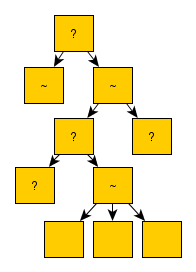
\includegraphics[width=0.35\textwidth]{Images/behaviour_tree.png}
\end{center}
\caption{Behavior Tree}
\label{pic3}
\end{figure}

Every behaviour has its own condition and an action. The algorithm starts at the root of the tree and at each levels examines the conditions of the behaviours. If a condition matches of a node, it executes the action. None of its siblings will be examined, but its children will. The algorithm is at as it follows:
\begin{verbatim}
    Make root node the current node
    While current node exists
        Run current node's condition
        If condition returns true
            Add node to execute list
            Make node's child current node
        Else
            Make node's sibling current node
    Run all behaviors on the execute list
\end{verbatim}

The real strenght of BTs is their simplicity \cite{BehaviourSelectionAlgorithms}. Since trees are stateless, the algorithm doesn't have to remember what behaviours were running and behaviours can be written without them being aware of each other. Extensibility is also a big plus, it is very easy to add more functionability at any given time.

But and now this is a big but, although BT algorithm is simple and powerful, its not always the best choice. The algorithm has to start at the root node every time a new behaviour is chosen, that means the running time is greatly impacted, in comparison to FSMs. Also, it deals with a lot of conditionals. Furthermore, memory is a problem as behaviours can loop with each other, however steps can be taken to deal with this problem.

\section{Scripting, the good and the bad}

Now we're about to talk the most controversial game AI that has existed. From it, it can come out to be the best game AI to ever be... or some of the worst. It all depends on its implementation.

However, to have a successful scripted AI, one must not fear it. Like any weapon, the soldier must first learn how to use to, to be useful with it. There are couple of ways to integrate scripting techniques into a game's architecture, but for the most part they compromise to two philosophies. Those rival points are "master" and "servant" ideologies \cite{ForbiddenScripting}, while both have their place, its very useful to consider which role scripts will play in a given game's implementation. 

\subsection{Master and Servant ideology}

To start off, to be successful into making a scripted AI, it is important to understand how important is a working system in the overall architecture of the game. Not just how it interacts with the AI, but in total game systems. Without a good architecture, scripts can't be effective, they produce huge amount of bugs, or even stop development.

So the most viable technique for scripted AI would be the master and servant approach. The master script would take care of the high-level aspects of the game, while the servant script would control the overall activity of the agents, or just create some kind of effects \cite{ForbiddenScripting}.  

\begin{itemize}
    \item Master scripts work best in two scenarios. The first one would be if in game already exists AI, and the scripting would be the "glue" that combines this techniques into a powerful model for agent behaviour. Even in the other scenario when its only the scripting technique, it can produce good results for different decision-making and planning techniques.
    \item Servant scripts are best effective when design requires a high degree in specificity in agent behaviour. So special case scenarios are created by the developers for each agent and this can have excellent results for ambient or "background" AI.
\end{itemize}

Games, would often tip themselves into one side or the other. It it dependant to a lot of circumstances: the experience of the developers, time and budget, the ratio of programmers to designers etc.


There is a stigma justified by negativities of players not enjoying games with scripted AI, which show little depth or veriety to their AI. But, with proper coordination between design and technical concerns of the project, scripted AI could become a powerful tool with a lot of depth.

Moreover, scripting should be used in combination with other techniques, due to over-reliance on scripts is why we get the shallow and unwanted AI. On an another page, developers must resist the urge to anticipate everything that a script might need to handle \cite{ForbiddenScripting}. This can be avoided with delegation, but the most important is having a chosen design early on and sticking to it, whether be it master and servant approach. When it comes to scripting, often simpler is better, instead of having to design overly complicated and intricate systems. Its better to stick on more flexible and creative solutions.

\section{Fuzzy Logic}

Fuzzy logic is a superset of conventional logic that has been extended to handle the concept of partial-truth values between the boolean dichotomy of true and false \cite{FuzzyAIGames}. It usually has its own components like fuzzy variables, fuzzy rules and fuzzy interface engines.

As well as the previous techniques, fuzzy logic has the goal of a simple design resulting in intelligent agents. Controlling a game character with fuzzy logic can be done easily due to suitable input and output values. 

Fuzzy logic is an extension of \emph{crisp logic} (conventional logic), there is the same as binary logic, the variable can be true or false \cite{FuzzyLogicBasedGameSystem}. In crisp logic, the variables can be from a set of two elements, while in fuzzy logic, the concept has been extended to handle partial-truth values between true and false. 

For example, the weapon range can be divided into melee, ranged or out of range as seen in \ref{pic4}.

\begin{figure}[h]
\begin{center}
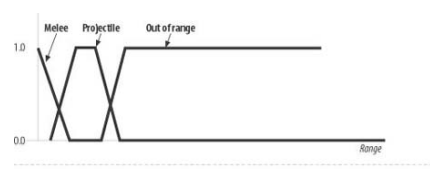
\includegraphics[width=0.53\textwidth]{Images/weapon_range.png}
\end{center}
\caption{Weapon range with Fuzzy Logic}
\label{pic4}
\end{figure}

Fuzzy logic brings a lot to the table when it come to game AI. It can help in NPC decision making or even weapon selection. With its benefits it can lead to an advanced AI with a pretty simple implementation. It can be even used in combination with FSMs (when transitioning from one state to another) and BTs (when branching out). For example, with conventional logic a car can only brake and accelerate, but with fuzzy logic it can be stated how much should the car brake and accelerate due to the gradual behaviour. 

\subsection{Pitfalls}

As good as fuzzy logic sounds till now, I have to talk about its downsides. Due to its knowledge-based nature, it requires a correct definition of input and output variables, as well as their relationships \cite{FuzzyAIGames}. Another downside, if the system of fuzzy logic is not designed carefully, it can lead to a lot of rules being checked at a given moment and sacrificing its advantage of a low computational cost.

In a video game, there can be many input variables to an agent's behaviour, each with their own number fuzzy sets. Because of this, the fuzzy rules can grow exponentially and it could even lead to combinatorial explosion \cite{CombinatorialBombing}.

\section{Flocking}

Flocking is a technique used to simulate intelligent movement of groups, the groups are called \emph{boids}. It is mostly used when NPCs need to move in a cohesive unit rather then independently. The genre of games that use this technique the most is RTS (Real-time strategy) games. The name "flocking" comes from flock of birds.

The one who's responsible for the flocking algorithm is Craig W Reynolds with his groundbreaking research \cite{FlocksReynolds}. His implementation is leaderless, is made in way that no boid leads the flock, they all just follow the group - which seems to have a mind of its own.

The flocking behaviour can be simulated by using three principles \cite{FlockingBehaviour}: 
\begin{itemize}
    \item Separation - Each boid knows the distances of its neighbors, so with that knowledge it tries to apply an repulsive force in the opposite direction to maintain distance from them. In a way, it is a collision avoidance within the flock.
    \item Cohesion - Computes the direction of the average position of the boids and tries to steer all the boids for them to be together as a group.
    \item Alignment - Keeps track of the average velocities and keeps check of the boids' velocities and tries to keep the average speed.
\end{itemize}

\begin{figure}[!htb]
\minipage{0.32\textwidth}
  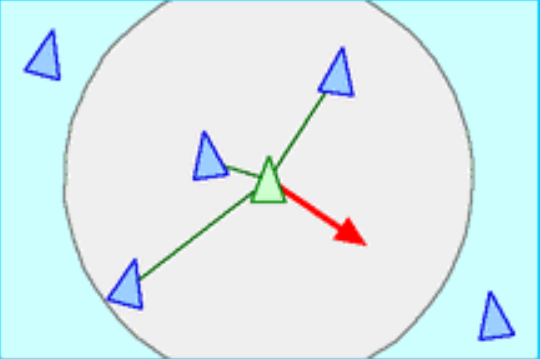
\includegraphics[width=\linewidth]{Images/separation.png}
  \caption{Separation}\label{fig:image1}
\endminipage\hfill
\minipage{0.32\textwidth}
  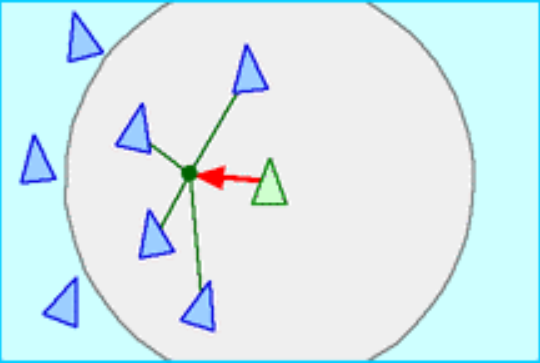
\includegraphics[width=\linewidth]{Images/cohesion.png}
  \caption{Cohesion}\label{fig:image2}
\endminipage\hfill
\minipage{0.32\textwidth}%
  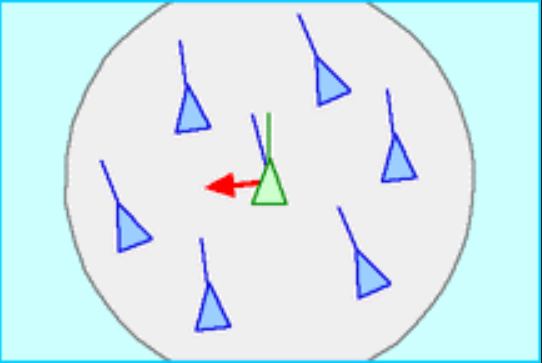
\includegraphics[width=\linewidth]{Images/alignment.png}
  \caption{Alignment}\label{fig:image3}
\endminipage
\label{pic5}
\end{figure}

The path of the boids which want to move is calculated by the A* pathfinding algorithm \cite{FOEAD2021507}. Its simple purpose is to find the shortest path from point A to point B. Its a well known method to use as a basis for pathfinding problems with its known  simplicty, efficency and modularity.

But, A* algorithm isn't fool proof, in many cases it would need a supplementary algorithm or a tweak to its core mechanics. Also, A* may find a path much quicker than other searches, but it does not ensure that the result will be the shortest path. Research shows that A* will have a correct result only 85\% of the time \cite{FOEAD2021507}. Overall, the traditional algorthm can't keep with the modern requirements of pathfinding, so game developers are needed to tweak and enforce it for adequate results.


\section{Genetics Algorithm}

A genetic algorithm is a probabilistic algorithm that generates an approximate solution based on Darwin’s Theory of Evolution \cite{GameAIGeneticAlg}. The basic gist of the algorithm is producing new offsprings from an existing population and then selecting the fittest offsprings from that populating for the next generations. This algorithm has been around for several decades so there may exist a lot of variations.

In this section, we'll take a look into a cetain genetic algorithm, which we need to define some terms for:

\begin{itemize}
    \item \emph{Gene} - Single parameter of search space
    \item \emph{Chromosome} - Collection of genes
    \item \emph{Individual} - Instantiated chromosome
    \item \emph{Population} - Collection of individuals
    \item \emph{Fitness} - Evaluation of an individual in our selected problem
    \item \emph{Crossover} - Process to create a new individual by breeding two
    \item \emph{Mutation} - Process to randomly change some genes to oppose local optima (solution that is optimal within a neighboring set of candidate solutions \cite{LocalOptimum}) 
    \item \emph{Generation} - One iteration of the Genetics Algorithm
\end{itemize}

\clearpage

Now, that we have defined some general terms we need for the algorithm, we can go ahead and get into it:

\begin{verbatim}
    Generate an initial random population
    Calculate fitness of every individual of the population
    Copy the individual over to the next generation
    Randomly mutate certain genes of individuals in the current generation
    From the mutated generation, choose pairs of individuals of certain 
        fitness to crossover
    If the number of maximum iterations of generation is not reached, 
        go the second line
\end{verbatim}

The best for a probabilistic algorithm is to iterate until there is no imporvements, but in the genetic algorithm we need to set up a number of iterations, because it always mutates.

The usage of genetics algorithms is immense, it can robustly and effectively search a poorly search space, when we have scarce knowledge. It is best for non-linear problems. The appeal of this algorithm comes from its elegance and simplicity for its power to discover good solutions for high-dimensional problems \cite{CurrentAIGames}.

And for the downsides, genetics algorithms require high computational and memory power, so it has big drawback when playing a game with it. Game developers mainly manage this by executing the algorithm when the game is not being played. In summary, its an effective algorithm based on evolution and natural selection and its used for learning and optimization.

\chapter{ML-Agents}
\label{ch3}

\section{Technologies}

To correctly use the ML-Agents toolkit we would need certain type of technologies. If we want to use the ML-Agents toolkit with Unity, we start with the Unity editor and Unity game engine \cite{UnitySoftware}. In the Unity editor, in the Package Manager, we should install "ML Agents".

After, we should have (or install) Python \cite{PythonManual} (I used python 3.9). With python pip we would need the packages pytorch and mlagents - For this step I chose to have a virtual environment, which is beneficial to have the proper versions and have the setting up part more organized.

Now, we are good to go, with the command \texttt{mlagents-learn} and Unity open we could freely proceed into the chapter with ease.

\section{Background}

After we've checked out some the key game AI that are used in the industry, I would like to present an open-source project The Unity Machine Learning Agents Toolkit or ML-Agents Toolkit. It is used for training intelligent agents through reinforcement learning, imitation learning, neuroevolution, or other ML methods through a simple-to-use Python API \cite{MLAgents}.

\subsection{Agents}

The technology of ML-Agents is mostly used for training Agents, which are basically NPCs, we can use variety of methods for the training. But, first we need to explain three entities of the game, which is the environment of the training.

\begin{itemize}
    \item \emph{Observations} - How the Agent sees the environment, the observations can be numeric and/or visual. Numeric observations can be some kind of attributes taken from the environment (they can be discrete or continuous), for the best results, the agent should have several continuous numerical observations. Visual observations are images generated from the cameras that are attached to our agent. The observations are separate from the environment, so that so that the agent can't get confused with data coming from the whole game/environment.
    \item \emph{Actions} - What can the agent do, same as the observations, the actions can be discrete or continuous. They can get as complex as the environment allows them to be.
    \item \emph{Reward signals} - How well the agent is doing, these signals don't have to be sent at every moment. The agent should be rewarded only when he does some action that is good, and punished when it does something bad. It should be noted that the rewarding is how the objective of the agent is communicated, so it should be set up in an optimal way for best results.
\end{itemize}

\subsection{Architecture}

The ML-Agents toolkit system works with 5 connected high-level components. And those are:

\begin{itemize}
    \item \emph{Learning environment} - is actually the Unity scene and all the game objects. This scene is used either for training or for testing environments, this is where the abovementioned Unity package ML Agents comes in handy. With it, the agents and their behaviours get defined.
    \item \emph{Python low-level API} - is interacting and manipulating the learning environment, it lives outside of the learning environment and interacts with it through the External communicator.
    \item \emph{External communicator} - connect the learning environment with the python low-level API, it actually lives in the learning environment.
    \item \emph{Python trainers} - contains all the ML algorithms, they are all contained in the python \texttt{mlagents} package.
    \item \emph{Gym wrapper} - common way in which ML researchers interact with learning environments is with the wrapper from openAI called gym.
\end{itemize}

\begin{figure}[h]
\begin{center}
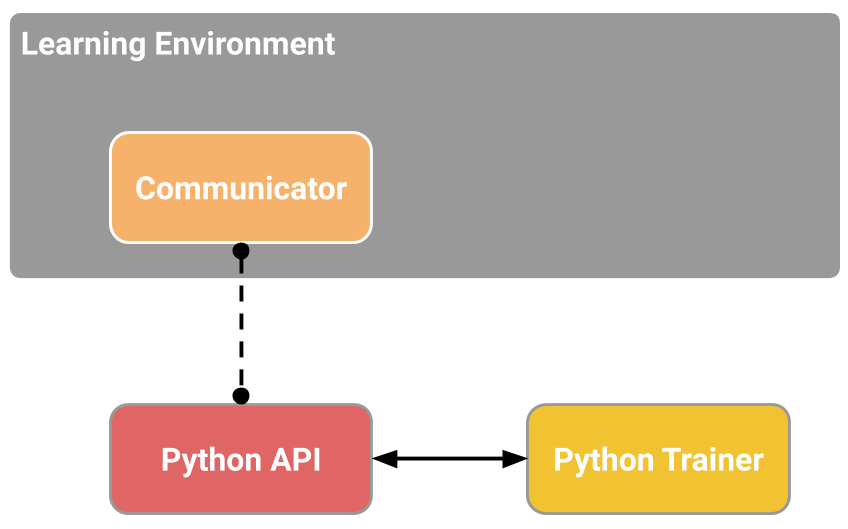
\includegraphics[width=0.7\textwidth]{Images/learning_environment_basic.png}
\end{center}
\caption{Simplified ML-Agents architecture \cite{MLAgents}}
\label{pic6}
\end{figure}


\clearpage

The learning environment in the Unity scene has two components:
\begin{itemize}
    \item \emph{Agent} - is linked to Game Object, handles the observations, actions and rewards.
    \item \emph{Behavior} - defines the attributes and number of actions the agent can take. It can be described as a function that takes the observations and rewards from the agent class and returns the actions. The behaviour can be one of three types:
    \begin{itemize}
        \item \emph{Learning} - not defined, about to be trained.
        \item \emph{Heuristic} - its defined by hard-coded rules, mainly is used for input for controlling the agent.
        \item \emph{Inference} - is already trained, and contains a already working and trained Neural Network file.
    \end{itemize}
    Basically, after a learning behaviour is trained, it becomes an inference behaviour.
\end{itemize}

\section{Examples and usages}

\subsection{Set up}

\chapter{Conclusion}
\label{ch4}



\cleardoublepage
\addcontentsline{toc}{chapter}{Literature}
\bibliography{literature}
\bibliographystyle{plainnat}

\end{document}